\subsection{Première partie du transitoire}
Le bain initial correspond à un bain oxyde avec une masse initiale de 10t, une température initiale de 2900 K et une composition en fractions massiques de 0.77 UO$_2$ - 0.12 Zr - 0.11 ZrO$_2$ (ratio molaire $R_{U/Zr}$ = 1.3 et degré  d'oxydation du zirconium $C_{Zr}$ = 30 \%). La puissance résiduelle massique est constante à $200$ W par kg d'uranium. La température de liquidus de l'oxyde est de 3000 K. Les corrélations d'échange de chaleur par les surfaces haute et latérale sont les corrélations Bali (voir~\cite{Bonnet1999} ou~\cite{Tourniaire2009a} pour plus de détails sur les corrélations). Enfin, un profil de flux plat est utilisé pour la distribution latérale de flux de la couche oxyde du bain pour la projection du flux sur les mailles de le croûte (voir section~\ref{sect:couplage}).

La croûte est divisée, tout au long du calcul, en 20 mailles. L'épaisseur de croûte ``résiduelle'' à son apparition est fixée à 5 mm. Une température constante et uniforme de 1600 K est imposée sur les parois extérieures de la croûte (seul le couplage entre le modèle de bain de corium et le modèle de croûte sont testés ici).

Le couplage entre le bain de corium et la croûte est résolu explicitement en temps avec un macro pas de temps de 100 s. Suffisamment de macro pas de temps sont calculés à partir de l'instant initial t = 0 s pour permettre au bain d'atteindre un état thermique quasi-stationnaire.

Durant les différentes étapes du transitoire, de la masse est échangée entre le bain de corium et sa croûte par solidification du bain ou fusion de la croûte. Une attention particulière a été portée pour que le volume de la croûte soit bien pris en compte pour le calcul du volume qu'occupe le bain de corium en fond de cuve de sorte que, le déplacement du niveau haut du bain associé à la solidification/fusion de la croûte (effet de densité) est faible.

La figure~\ref{fig:mass_balance} donne les masses du bain de corium et la masse globale de croûte.
\begin{figure}[H]
\centering
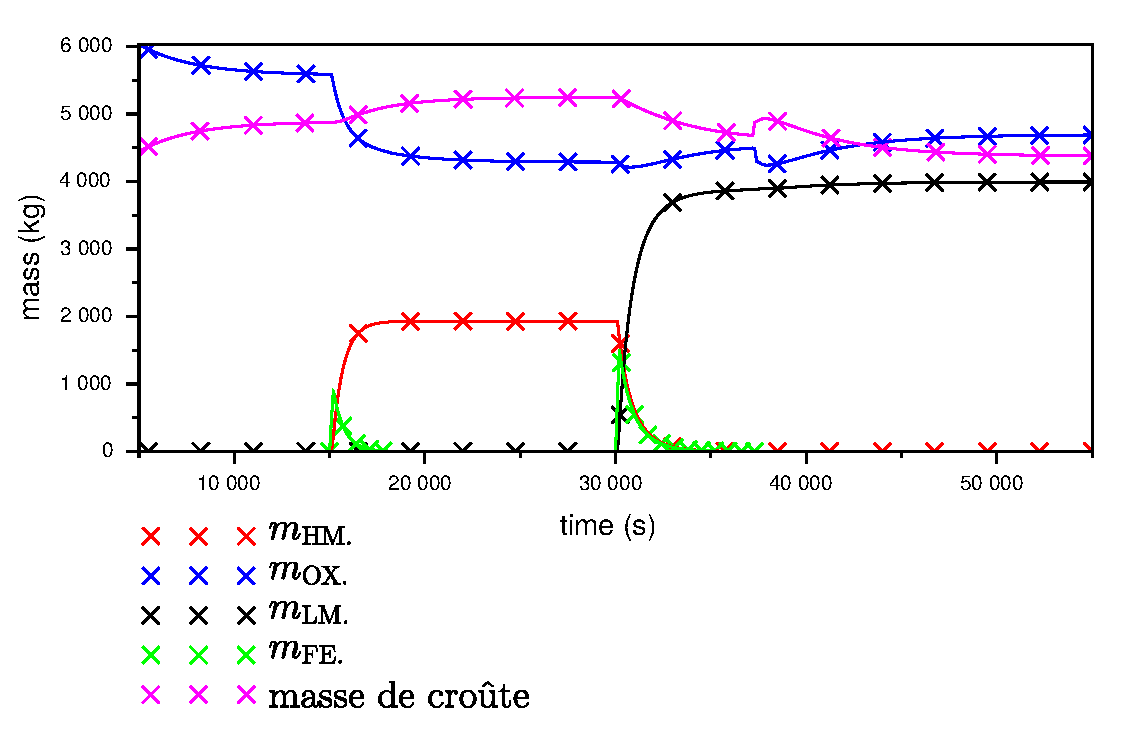
\includegraphics[width=0.85\textwidth, keepaspectratio=true]{Figures/mass_balance.eps}\\
\caption{Masses de la croûte et de la couche oxyde du bain}
\label{fig:mass_balance}
\end{figure}
À chaque macro pas de temps du calcul et en fin de calcul, \emph{on vérifie bien la conservation de la masse globale du système}.

De la même manière, de l'énergie est échangée entre le bain de corium et la croûte et \emph{on vérifie la conservation globale de l'énergie du système}. La figure~\ref{fig:thermal_balance} donne les différentes puissances d'intérêt du bain de corium et de la croûte au cours du transitoire : les puissances évacuées par la surface latérale de la couche oxyde du bain $\bar{\phi}^{lat}_\textrm{OX.}S^{lat}_\textrm{OX.}$ et par sa surface supérieure $\bar{\phi}^{up}_\textrm{OX.}S^{up}_\textrm{OX.}$, la puissance résiduelle de la couche oxyde du bain $Q_\textrm{OX.}$ ainsi que la somme des puissances résiduelles $Q_{C_j}$ des mailles $C_j$ de la croûte, et enfin la somme des puissances $\bar{\phi}_{j,ext}S_{j,ext}$ évacuées par la surface extérieure $\gamma_{ext}$ des mailles $C_j$ de la croûte.
\begin{figure}[H]
\centering
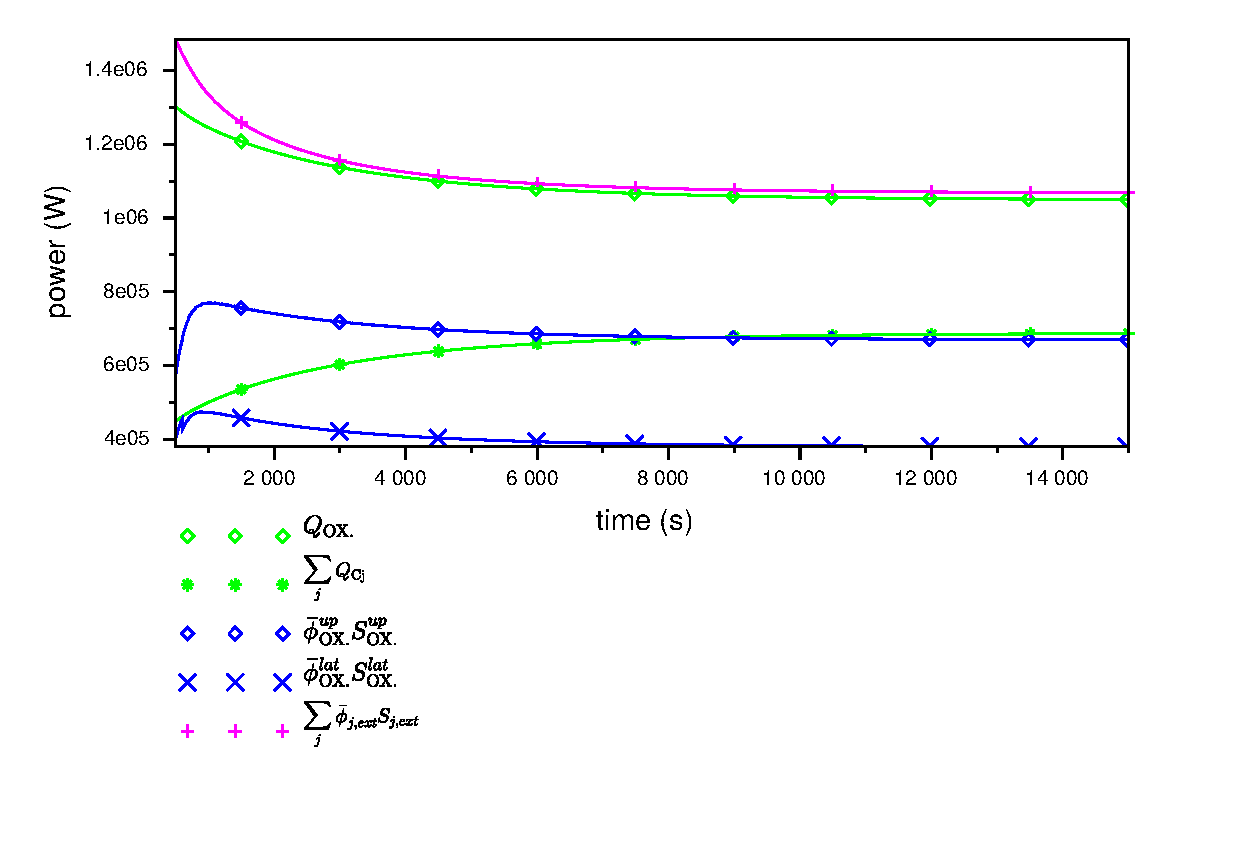
\includegraphics[width=0.85\textwidth, keepaspectratio=true]{Figures/thermal_balance.eps}\\
\caption{Puissances d'intérêt du système bain de corium et croûte}
\label{fig:thermal_balance}
\end{figure}
La conservation de l'énergie peut être vérifiée graphiquement dans la figure~\ref{fig:thermal_balance} à l'état quasi-stationnaire atteint. Pour t=15 000 s, on vérifie bien que
\begin{equation}
\bar{\phi}^{up}_\textrm{OX.}S^{up}_\textrm{OX.} + \bar{\phi}_{j,ext}S_{j,ext} = Q_\textrm{OX.} + \sum_j Q_{C_j}.
\end{equation}

Durant le transitoire du couplage, les mailles de la croûte sont directement en était de solidification (voir la section~\ref{sect:thermique} pour la description des différents états solidification, conduction et fusion). La croûte se solidifie jusqu'à atteindre un état quasi-stationnaire de solidification (voir figure~\ref{fig:croutes_1}) et, conformément au choix d'un profil uniforme de flux, l'épaisseur de la croûte est, elle aussi uniforme.

\begin{figure}[H]
\centering
\includegraphics[width=\textwidth, keepaspectratio=true]{Figures/coriumCrust_100.png}\\
\includegraphics[width=\textwidth, keepaspectratio=true]{Figures/coriumCrust_15000.png}
\caption{Croûte à t = 100 s (en haut) et à t = 15 000 s (en bas). \textit{L'indice dans la maille $C_j$ donne la couche de bain en face de celle-ci : 1 $\Leftrightarrow$ OX., -1 $\Leftrightarrow$ Vide}}
\label{fig:croutes_1}
\end{figure}

\subsection{Seconde partie du transitoire}
\iffalse
Une condition adiabatique est imposée en surface haute de la couche d'acier liquide hors équilibre du bain (FE.). Un profil de flux plat est utilisé pour la distribution latérale de flux de toutes les couches du bain pour la projection des flux des différentes couches du bain sur les mailles de le croûte (voir section~\ref{sect:couplage}). Enfin, les caractéristiques utiles des différentes couches du bain sont détaillées dans le tableau~\ref{tab:caracteristiques_couches_bain}, en particulier les températures de ``liquidus'' des couches ainsi que les corrélations de flux de chaleur utilisées pour le calcul des puissances latérales $\phi S$ (voir~\cite{Bonnet1999} ou~\cite{Tourniaire2009a} pour plus de détails sur les corrélations).

Une fois que ce bain oxyde et sa croûte ont atteint un régime permanent, une coulée d'acier liquide est considérée. La masse d'acier ajoutée a été selectionnée vis-à-vis du seuil d'inversion de stratification du bain\footnote{correspondant à quantité d'acier dans la bain permettant le passage d'un état d'équilibre thermochimique composé d'une couche métallique lourde en dessous d'une couche oxyde vers un équilibre composé d'une couche oxyde en dessous d'une couche métallique légère} afin d'amener le bain vers un équilibre à deux couche : une couche métallique lourde surmontée d'une couche oxyde. Les caractéristiques de cette coulée (temps de début et de fin, masse, température et composition) sont détaillés dans le tableau~\ref{tab:coulees_acier}. 
\begin{table}
	\centering
	\begin{tabular}{ccccc} 
	\hline
	$t_{\text{début}}$ (s) &  $t_{\text{arrêt}}$ (s) & Débit (kg/s) & T (K) & Composition\\
	\hline
	15 000 & 15 200 & 5 & 1605 & 0.687 Fe - 0.208 Cr - 0.106 Ni\\
	\hline
	\end{tabular}	
	\caption{Coulée d'acier liquide imposée pour le test} 
	\label{tab:coulees_acier}
\end{table}
A l'issue de cette coulée, un temps de simulation suffisamment long a été imposé pour permettre au bain d'atteindre un état thermique et thermochimique quasi-stationnaire. 

\begin{figure}[H]
\centering
\includegraphics[width=\textwidth, keepaspectratio=true]{Figures/croute_15000.png}\\
\includegraphics[width=\textwidth, keepaspectratio=true]{Figures/croute_15100.png}\\
\includegraphics[width=\textwidth, keepaspectratio=true]{Figures/croute_16000.png}\\
\includegraphics[width=\textwidth, keepaspectratio=true]{Figures/croute_18000.png}\\
\includegraphics[width=\textwidth, keepaspectratio=true]{Figures/croute_30000.png}\\
\caption{De haut en bas, croûte à t = 15 000 s, t=15 100 s, t=16 000 s, t=18 000 s, t=30 000 s (état quasi-stationnaire du bain HM./OX.). \textit{L'indice dans la maille $C_j$ donne la couche de bain en face de celle-ci : 0 $\Leftrightarrow$ HM., 1 $\Leftrightarrow$ OX.}}
\label{fig:croutes_2}
\end{figure}

Lors de la seconde partie du transitoire, la couche de métal lourd apparaît suite à une coulée d'acier liquide (voir tableau~\ref{tab:coulees_acier}). La figure~\ref{fig:croutes_2} donne les différents états de la croûte durant ce transitoire.

Entre t=15 000 s et t=15 100 s, une maille de croûte apparaît en face d'une couche d'acier liquide (à une hauteur h $>$ 0.42 m) provenant de la coulée et le maillage de la croûte oxyde passe de 20 mailles (à t=15 000s) à 19 mailles (à t=15 100s). Cette maille de croûte acier apparaît avec une épaisseur initiale de 5 mm mais fond presque instantanément et disparaît. Ensuite, la couche de métal lourd s'épaissit et le volume du bain composé des couches HM. et OX. augmente du fait du transfert de masse depuis la couche FE. Par conséquent, une croûte oxyde apparaît au fur et à mesure que la couche OX. monte (voir les figures à t=16 000 s et t=18 000 s). Par ailleurs, comme attendu, en face de la couche HM., le flux latéral est évacué par conduction (sans évolution de la croûte oxyde). A t=30 000 s, la thermochimie et la thermique du bain se sont stabilisées et la croûte n'évolue plus : on retrouve bien les profils plats de flux de bain projetés sur les mailles de la croûte.
\fi

\subsection{Tests de vérification à venir}

